\section{PairUAV: sampling, screening, unscreened pairs, release}
\label{sec:dataset}

The reviewers ask for the sampling ranges of Sec.~3.2, the screening criterion and its statistics, results on pairs that were not screened, the distribution of flight heights and tilts, and a release plan.

\begin{table}[t]
\centering
\caption{\textbf{Statistics of PairUAV} over 1{,}412 buildings.}
\label{tab:dataset}
\footnotesize
\setlength{\tabcolsep}{3.5pt}
\resizebox{\columnwidth}{!}{%
\begin{tabular}{@{}lrrrrrl@{}}
\toprule
& min & 5\% & 50\% & 95\% & max & \\
\midrule
\multicolumn{7}{@{}l}{\emph{Cameras} (211{,}800)}\\
Height above terrain & 203.5 & 204.6 & 220.0 & 235.4 & 236.5 & m \\
Tilt $\psi$ & 0.0 & 2.2 & 22.5 & 42.7 & 45.0 & $^\circ$ \\
Horizontal offset from the anchor & 0.0 & 2.9 & 12.6 & 18.9 & 21.2 & m \\
\midrule\multicolumn{7}{@{}l}{\emph{Selected pairs} (1{,}412{,}000)}\\
Baseline $\|\dpv\|$ & 0.3 & 9.1 & 20.1 & 32.5 & 38.9 & m \\
$|\Delta x|$ & 0.0 & 0.7 & 7.6 & 14.0 & 15.0 & m \\
$|\Delta y|$ & 0.0 & 0.7 & 7.6 & 14.0 & 15.0 & m \\
$|\Delta z|$ & 0.0 & 1.2 & 15.2 & 29.9 & 33.0 & m \\
$|\dpsi|$ & 0.0 & 2.2 & 20.8 & 35.9 & 44.9 & $^\circ$ \\
$|\dth|$ & 0.0 & 4.5 & 91.2 & 167.1 & 176.0 & $^\circ$ \\
\midrule\multicolumn{7}{@{}l}{\emph{All candidate pairs} (31{,}558{,}200)}\\
Baseline $\|\dpv\|$ & 0.1 & 7.9 & 19.9 & 33.6 & 52.3 & m \\
$|\Delta x|$ & 0.0 & 0.7 & 8.7 & 24.9 & 30.0 & m \\
$|\Delta z|$ & 0.0 & 0.7 & 9.6 & 27.4 & 33.0 & m \\
$|\dpsi|$ & 0.0 & 1.3 & 13.3 & 35.0 & 45.0 & $^\circ$ \\
$|\dth|$ & 0.0 & 4.7 & 93.9 & 169.1 & 179.6 & $^\circ$ \\
\midrule\multicolumn{7}{@{}l}{\emph{Screening statistics stored with the selected pairs}}\\
SIFT matches & 20 & 64 & 373 & 1299 & 3028 &  \\
Inliers & 20 & 57 & 361 & 1282 & 3027 &  \\
Inlier ratio & 0.37 & 0.86 & 0.97 & 0.99 & 1.00 &  \\
Hull fraction of the inliers & 0.01 & 0.09 & 0.24 & 0.57 & 0.96 &  \\
Occupied cells of a $4{\times}4$ grid & 4 & 4 & 6 & 13 & 16 &  \\
\bottomrule
\end{tabular}}
\end{table}


\subsection{Sampling of the cameras}

For each building, an anchor point is taken from its University-1652 tour, and 150 cameras are placed around it: horizontally within $\pm15$\,m of the anchor in east and north, at a height between \dsHmin{} and \dsHmax\,m above the terrain at the anchor, with headings over the full circle, tilts between $0^\circ$ and $45^\circ$ from the nadir, and zero roll. The draws are stratified, so that every building spans the ranges in the same way: tilts are spread evenly, heights fall in three bands and headings in fifteen bands of about $8^\circ$ spaced by $24^\circ$ (\cref{fig:dataset}). The images are rendered at $3686{\times}2073$ pixels. \Cref{tab:dataset} gives the resulting statistics over the \dsBuildings{} buildings (\dsCameras{} images) available to us at the time of the experiments.

Two consequences should be stated plainly. First, all cameras of PairUAV fly at \dsHmean$\,\pm\,$\dsHstd\,m above the ground. This regularity is what the flight-height cue of \cref{sec:cands} exploits, and it is why a single calibrated constant recovers the metric scale on this benchmark (\cref{sec:inventory}); a dataset with a wide range of flight heights would require the height as an input, as in \cref{sec:real}. Second, a displacement of one metre corresponds to about 15 pixels on the ground at full resolution: the benchmark measures metre-level alignment from high-altitude views, not close-range flight.

\begin{figure}[t]
\centering
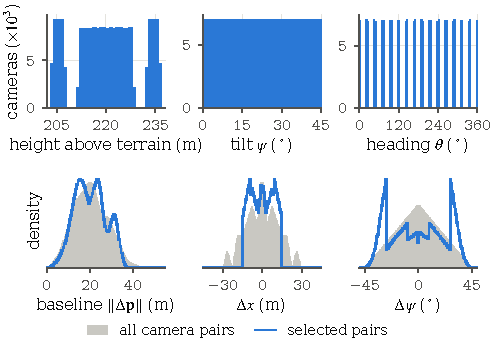
\includegraphics[width=\linewidth]{figures/fig_dataset.pdf}
\caption{\textbf{Camera and pair statistics of PairUAV.} Top: height above the terrain, tilt and heading of the cameras. Bottom: baseline length and pose differences of all camera pairs of a building (grey) and of the selected pairs (line).}
\label{fig:dataset}
\end{figure}

\subsection{Screening and selection of the pairs}

The 150 cameras of a building give \dsCand{} ordered pairs. The released pairs are obtained in three steps.

\noindent\textbf{Range.} All released pairs satisfy $|\Delta x|,|\Delta y|\le15$\,m, whereas the candidates reach 30\,m; the other three differences span the sampling ranges. \dsInRange\% of the candidate pairs lie within the ranges of the released ones.

\noindent\textbf{Visual screen.} Every released pair carries the statistics of an automatic screen, which we report from the metadata: SIFT matches filtered by a mutual ratio test, a fundamental matrix fitted with MAGSAC, the number of inliers, their ratio, the fraction of the image covered by their convex hull, and the number of occupied cells of a $4{\times}4$ grid. All released pairs have at least \dsMinInl{} inliers spread over at least \dsMinCells{} cells; the median pair has \dsInlMed{} inliers with an inlier ratio of \dsInlRatioMed, and \dsInlLtHundred\% of the pairs have fewer than 100 inliers (\cref{tab:dataset}). \todoauthors{Sec.~3.2 states that human annotators screened candidate pairs. Please provide the number of annotators, the agreement criterion, the number of candidate pairs shown and the rejection rate, and how the manual screen relates to the automatic one recorded in the metadata; none of this can be recovered from the released files, and we leave it blank rather than guess.}

\noindent\textbf{Balancing.} From the pairs that pass, 1{,}000 are selected per building, jointly over groups of five buildings (\dsGroups{} groups), with equal counts in five equal-width bins of each of the five pose differences. The released pairs are \dsSelFrac\% of all candidate pairs and \dsSelOfInRange\% of those within range. Their baselines range up to \dsDistMax\,m with a median of \dsDistMed\,m; 1\% are shorter than \dsDistPone\,m (\cref{tab:dataset}, \cref{fig:dataset}).

\subsection{Results on unscreened pairs}
\label{sec:unfiltered}

The reviews ask how the method performs on pairs that did not pass the selection. We use the \unN{} unscreened pairs of \cref{sec:unscreened}: four ordered pairs per test building, drawn uniformly from all $150{\times}149$ camera pairs, with labels recomputed from the camera poses. Of these pairs, \ufInX\% and \ufInY\% lie within the $\pm15$\,m of the released pairs in $\Delta x$ and in $\Delta y$ (\unInside\% in both), and our re-implementation of the visual screen, which accepts \ufProxyPass\% of the released pairs, accepts \unScreenPass\% of them.

\begin{table}[t]
\centering
\caption{\textbf{Unscreened pairs by overlap of the two ground footprints} (pairs of \cref{tab:unscreened}; refined stage unless stated, camera frame).}
\label{tab:overlap}
\footnotesize
\setlength{\tabcolsep}{4pt}
\begin{tabular}{@{}lccccc@{}}
\toprule
& Share & \SRd & \SRe & \SRe & EPE med. \\
Overlap & (\%) & (\%) & coarse & refined & (m) \\
\midrule
$<$ 0.02 & 23.1 & 7.8 & 0.4 & 0.4 & 21.32 \\
0.02-0.2 & 23.3 & 61.5 & 24.1 & 47.8 & 1.10 \\
0.2-0.4 & 24.0 & 80.9 & 68.7 & 78.8 & 0.53 \\
0.4-0.6 & 19.0 & 82.7 & 78.2 & 82.3 & 0.46 \\
$\geq$ 0.6 & 10.7 & 91.1 & 83.1 & 91.1 & 0.41 \\
\bottomrule
\end{tabular}
\end{table}


Over all unscreened pairs the refined stage reaches \unSiiSRd\% \SRd{} and \unSiiSRe\% \SRe{} in the camera frame (\cref{tab:unscreened}), against \SiiCamSRd\% and \SiiCamSRe\% on the released test pairs. On the unscreened pairs that lie within the released ranges and pass the screen it reaches \unInSiiSRd\% and \unInSiiSRe\%: the released pairs are representative of the pairs with these two properties, and the difference comes from the others. The decisive factor is the overlap of the two ground footprints (\cref{tab:overlap}). Pairs whose footprints overlap by less than 2\%, which are \unNoOverlap\% of all camera pairs of a building, cannot be solved by any method of \cref{tab:unscreened}; above 20\% of overlap the success is at the level of the released pairs; in between, the refinement doubles the endpoint success of the coarse stage. DreamNav returns an estimate for every pair, including those without common content. The numbers of the main paper therefore describe pairs that overlap, as its dataset section states, and a deployed system needs a test that rejects the others; the number of inliers, which is zero in the median for the pairs of the first row, is an obvious candidate that we have not evaluated.

\subsection{Release}

The footnote of the abstract commits to releasing the dataset and the code upon publication. The release will contain: the rendered images; the pose of every camera; the pair lists with their five labels and screening statistics, including the lists of unscreened pairs used in \cref{sec:unfiltered}; the building-level training and test splits; the evaluation code with the metric definitions of \cref{sec:metrics}, so that the range-based and the endpoint-based success rates are both reported; and the code and fitted models of DreamNav, including the scripts that produce every table of this document. \todoauthors{Please confirm the hosting, the licence of the rendered imagery, and whether the anonymised package can be linked for the reviewers.}
